\documentclass{scrartcl}
\usepackage[utf8]{inputenc}
\usepackage{tikz}
\usetikzlibrary{arrows,decorations.pathmorphing,backgrounds,fit,positioning,shapes.symbols,chains,shapes.geometric,shapes.arrows,calc}

\begin{document}

    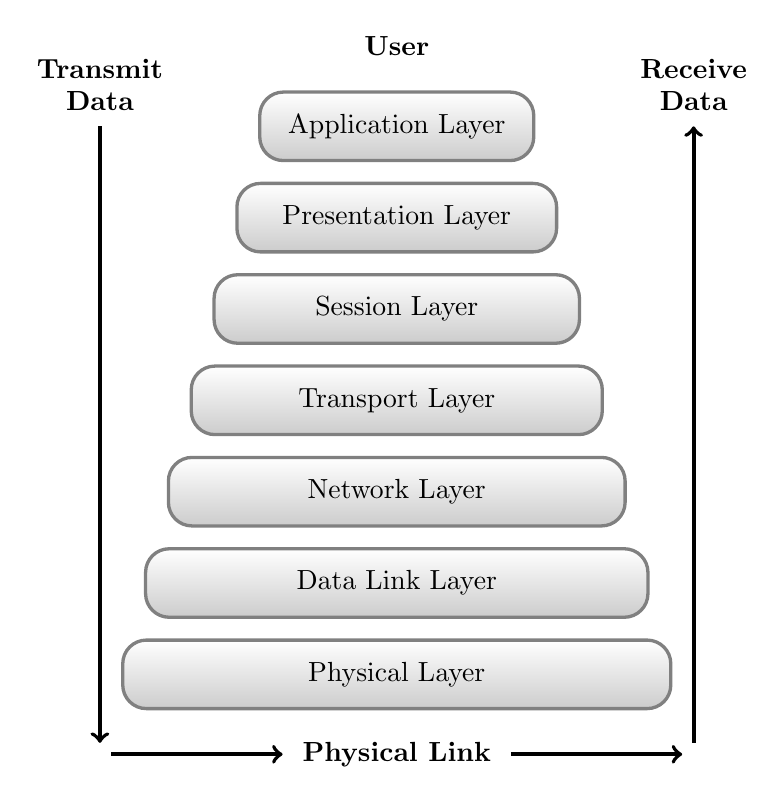
\begin{tikzpicture}[scale=0.58]
    
        \draw[rounded corners=3mm,very thick,draw=black!50,top color=white,bottom color=black!20] (-3,0) rectangle (3,-1.5);
        \draw[rounded corners=3mm,very thick,draw=black!50,top color=white,bottom color=black!20] (-3.5,-2) rectangle (3.5,-3.5);
        \draw[rounded corners=3mm,very thick,draw=black!50,top color=white,bottom color=black!20] (-4,-4) rectangle (4,-5.5);
        \draw[rounded corners=3mm,very thick,draw=black!50,top color=white,bottom color=black!20] (-4.5,-6) rectangle (4.5,-7.5);
        \draw[rounded corners=3mm,very thick,draw=black!50,top color=white,bottom color=black!20] (-5,-8) rectangle (5,-9.5);
        \draw[rounded corners=3mm,very thick,draw=black!50,top color=white,bottom color=black!20] (-5.5,-10) rectangle (5.5,-11.5);
        \draw[rounded corners=3mm,very thick,draw=black!50,top color=white,bottom color=black!20] (-6,-12) rectangle (6,-13.5);
    
        \node[] at (0, -0.75) {Application Layer};
        \node[] at (0, -2.75) {Presentation Layer};
        \node[] at (0, -4.75) {Session Layer};
        \node[] at (0, -6.75) {Transport Layer};
        \node[] at (0, -8.75) {Network Layer};
        \node[] at (0, -10.75) {Data Link Layer};
        \node[] at (0, -12.75) {Physical Layer};
    
        \node[] at (0, 1.0) {\textbf{User}};
        
        \node[] at (-6.5, 0.5) {\textbf{Transmit}};
        \node[] at (-6.5, -0.2) {\textbf{Data}};
       
        \node[] at (6.5, 0.5) {\textbf{Receive}};
        \node[] at (6.5, -0.2) {\textbf{Data}};
       
        \node[] at (0, -14.5) {\textbf{Physical Link}};    
    
        \draw[->, line width=0.5mm] (-6.5,-0.75) -- (-6.5,-14.25) ;        
        \draw[->, line width=0.5mm] (-6.25,-14.5) -- (-2.5,-14.5) ;
        \draw[->, line width=0.5mm] (2.5,-14.5) -- (6.25,-14.5) ;
        \draw[->, line width=0.5mm] (6.5,-14.25) -- (6.5,-0.75) ;
        
    \end{tikzpicture}
 \end{document}
